Ein GALS System -- GALS steht für "`Globally asynchronous, locally synchronous"' -- besteht aus mehreren synchronen Komponenten, die asynchron miteinander kommunizieren.
Die synchronen Komponenten lassen sich dabei als Mealy-Automaten auffassen.
In einem Mealy-Automaten hängt die Ausgabe sowohl von der Eingabe als auch dem aktuellen Zustand ab\cite{Mealy}.
Mealy-Automaten sind so allgemein formuliert, dass sich jedes in einem synchronen Formalismus formulierte Modell in einen bisimularen Mealy-Automaten transformieren lässt.
Ein Beispiel für einen Mealy-Automaten ist in Abbildung \ref{fig:mealy} dargestellt.
Transitionen sind hier in der Form $i/o$ angegeben, wobei $i$ die Eingabe und $o$ die Ausgabe bezeichnen.
\begin{figure}[h]
  \centering
  \begin{tikzpicture}
  [initial text=,
  shorten >=1pt,
  >=stealth',
  every state/.style={draw=d1,very thick,fill=d1!40}
  ]
  \node[state,initial] (q0) at (0,2) {$q_0$};
  \node[state] (q1) at (2,2) {$q_1$};
  \node[state] (q2) at (1,0) {$q_2$};
  
  \path[->] (q0) edge[bend left] node[above] {$a/b$} (q1)
                 edge node[left] {$b/a$} (q2)
            (q1) edge node[below] {$a/c$} (q0)
                 edge[bend left] node[right] {$b/a$} (q2)
            (q2) edge node[left] {$a/b$} (q1)
                 edge[loop below] node {$b/c$} (q2);
\end{tikzpicture}

  \caption{Mealy-Automat}
  \label{fig:mealy}
\end{figure}

Ein Schritt im Automaten bedeutet, dass das aktuelle Eingabe-Symbol gelesen wird und die Transition gewählt wird, die vom aktuellen Zustand ausgeht und mit dem aktuellen Eingabe-Symbol übereinstimmt.
Das Ziel der Transition ist der neue aktuelle Zustand des Automaten und das Ausgabe-Symbol der Transition wird zur Ausgabe hinzugefügt.
Der Beispiel-Automat in Abbildung \ref{fig:mealy} hat also beispielsweise die folgende Ablauf-Sequenz:

\[ \xymatrix {
     q_0\ar[r]^a &  q_1 \ar[r]^a & q_0 \ar[r]^a & q_1 \ar[r]^b & q_2\ar[r] & \dots
   } \]
Der Automat transformiert damit die Eingabe "`$aaab\dots$"' in die Ausgabe "`$bcba\dots$"'.
Der Beispiel-Automat verwendet als Ein- und Ausgabe-Symbole Zeichen und stellt damit einen Aus- und Eingabekanal zur Verfügung.
Benutzt man stattdessen $n$-Tupel als Eingabe und $m$-Tupel als Ausgaben, erhält man einen Automaten, der $n$ Eingabe- und $m$ Ausgabe-Kanäle bietet.
In jedem Schritt wird dann aus jedem Eingabekanal ein Zeichen gelesen und in jeden Ausgabekanal eins geschrieben.

Für die vollständige Beschreibung eines Mealy-Automaten mit Kanälen ist die Repräsentation durch Tupel ausreichend, für eine übersichtliche Notation und Darstellung jedoch nicht geeignet, da die Anzahl der aufzuschreibenden Transitionen exponentiell mit der Anzahl der Eingabe-Kanäle wächst\footnote{Hat man $n$ Eingabe-Kanäle, die jeweils $m$ verschiedene Zeichen enthalten können, so benötigt jeder Zustand $m^n$ ausgehende Transitionen, da der Automat für jede Eingabe eine gültige Transition aufweisen sollte.}.
Daher ist es sinnvoll, für die Spezifikation von Mealy-Automaten die Tupel-Komponenten mit Variablen zu benennen und Bedingungen (engl. \emph{conditions}) über diese Variablen an die Transitionen zu schreiben.
Eine Bedingung ist hierbei eine boolesche Formel, die nur die Variablen der Tupelkomponenten enthält.
Ist die Formel für eine Belegung der Variablen wahr, so gilt die Transition auch für das entsprechende Tupel.

Benennt man beispielsweise die Komponenten der Tupel $\mathbb{N}\times\mathbb{B}\times\mathbb{B}$ mit $\alpha$, $\beta$ und $\gamma$, so beschreibt die Bedingung $\alpha=3\land\gamma=0$ die Tupel $(3,0,0)$ und $(3,1,0)$.
Eine Transition $\alpha=3\land\gamma=0/(1,2)$ beschreibt also eigentlich die Transitionen $(3,0,0)/(1,2)$ und $(3,1,0)/(1,2)$.
Diese Art der Notation ist hilfreich, wenn für eine Transition die Werte von bestimmten Kanälen keine Rolle spielen.
Abbildung \ref{fig:mealy2} zeigt einen Beispiel-Automaten, der Tupel der Form $\mathbb{B}\times\mathbb{N}$ als Eingaben verwendet.

\begin{figure}[h]
  \centering
  \begin{tikzpicture}
  [initial text=,
  shorten >=1pt,
  >=stealth',
  every state/.style={draw=blue!50,very thick,fill=blue!20}
  ]
  \node[state,initial] (q0) at (0,0) {$q_0$};
  \node[state] (q1) at (3,0) {$q_1$};
  
  \path[->] (q0) edge[bend left] node[above] {$\mathit{on}\land x<5/1$} (q1)
                 edge[loop above] node {$\lnot\mathit{on}\lor x\geq 5/3$} (q0)
            (q1) edge[bend left] node[below] {$x\geq 5/0$} (q0)
                 edge[loop right] node {$x<5/2$} (q1);
\end{tikzpicture}

  \caption{Mealy-Automat mit Bedingungen}
  \label{fig:mealy2}
\end{figure}

Um ein GALS-System zu erstellen, kann man nun die Ausgabekanäle von Automaten mit den Eingabekanälen von anderen Automaten verbinden und so ein Netzwerk aus Mealy-Automaten erhalten.
Ist die Eingabe eines Automaten mit einer Ausgabe verbunden, so verwendet der Automat immer die letzte produzierte Ausgabe des verbundenen Automaten als Eingabesymbol.

Abbildung \ref{fig:mealy3} zeigt ein solches System.
Das Gesamtsystem hat sämtliche unverbundenen Aus- und Eingaben als Aus- und Eingaben.
Ein Schritt des Gesamtsystems wird nun durch einen Schritt eines beliebigen Mealy-Automaten realisiert.
Durch diese Eigenschaft wird das GALS-System nicht-deterministisch und asynchron.
Ein Problem ergibt sich nun, wenn die Quelle einer Verbindung noch keinen Schritt durchgeführt hat: in diesem Fall gibt es keinen letzten Wert für die Verbindung und die Eingabe des Ziel-Automaten ist undefiniert.
Dieser Fall kann durch die Definition von Default-Werten oder durch das Verbot, Schritte mit Automaten durchzuführen, deren Eingaben (teilweise) undefiniert sind gelöst werden.
\begin{figure}[h]
  \centering
  \begin{tikzpicture}
  [initial text=,
  shorten >=1pt,
  >=stealth',
  every state/.style={draw=blue!50,very thick,fill=blue!20}
  ]
  %\node[draw,red!50,fill=red!20,very thick,minimum height=1cm,minimum width=4cm] (c1) at (0.25,0.5) {};
  
  %\draw[color=red!50,fill=red!20,very thick] (-1,1) -- (-1,-1) -- (3,-1) -- (3,1) -- (-1,1);
  \path[draw,red!50,fill=red!20,very thick] (-1,1) rectangle (2.6,-1);
  \path[draw,red!50,fill=red!20,very thick] (2.6,-1) rectangle (3.3,1);
  \node[state,initial] (q0) at (0,0) {$q_0$};
  \node[state] (q1) at (2,0) {$q_1$};
  \path[->] (q0) edge[bend left] node[above] {$/0$} (q1)
            (q1) edge node[below] {$/1$} (q0);
  \node at (2.3,0.7) {$P_1$};
  \node (tout) at (2.95,0) {out};
  \begin{scope}[shift={(5.5,-0.15)}]
    \path[draw,red!50,fill=red!20,very thick] (-1.2,-1.8) rectangle (4,0.8);
    \path[draw,red!50,fill=red!20,very thick] (-1.2,-1.8) rectangle (-1.8,-0.5);
    \path[draw,red!50,fill=red!20,very thick] (-1.2,-0.5) rectangle (-1.8,0.8);
    \path[draw,red!50,fill=red!20,very thick] (4,-1.8) rectangle (4.7,0.8);
    \node[state,initial] (p0) at (0,0) {$q_0$};
    \node[state] (p1) at (3,0) {$q_1$};
  
    \path[->] (p0) edge node[above] {$\mathit{on}\land x<5/1$} (p1)
                   edge[loop below] node {$\lnot\mathit{on}\lor x\geq 5/3$} (p0)
              (p1) edge[bend left] node[below] {$x\geq 5/0$} (p0)
                   edge[loop below] node {$x<5/2$} (p1);
    \node at (-1.5,-1.15) {x};
    \node (ton) at (-1.5,0.15) {on};
    \node at (3.7,0.5) {$P_2$};
    \node at (4.35,-0.5) {res};
  \end{scope}
  \path[->,thick] (tout) edge (ton);
\end{tikzpicture}

  \caption{Aus Mealy-Automaten zusammen gesetztes GALS-System}
  \label{fig:mealy3}
\end{figure}

Das in Abbildung \ref{fig:mealy3} gezeigte System hat also nur die Eingabe $x$ und die Ausgabe $\mathit{res}$.
Der Gesamtzustand des Systems ist nun durch den Zustand der Verbindungen und den aktuellen Zustand der Prozesse definiert.
Der Startzustand des abgebildeten Systems kann also beispielsweise durch $(p_0,q_0,\bot)$ dargestellt werden, wobei $\bot$ angibt, dass die Verbindung zwischen $\mathit{out}$ und $\mathit{on}$ undefiniert ist.
Eine Transition wird dargestellt durch ein Tupel, dass die Ein- und Ausgaben des Systems sowie den Mealy-Automaten, der den aktuellen Schritt durchführt, enthält.
Die Transition $(4,P_1)/3$ gibt also beispielsweise an, dass die Eingabe $x$ den Wert $4$, die Ausgabe $\mathit{res}$ den Wert $3$ besitzt und der Automat $P_1$ einen Schritt durchführt hat.
Das resultierende Transitionssystem für das GALS-System aus Abbildung \ref{fig:mealy3} ist beispielsweise in Abbildung \ref{fig:gals_trans} dargestellt.

\begin{figure}[h]
  \centering
  \begin{tikzpicture}
  [initial text=,
  shorten >=1pt,
  >=stealth',
  every state/.style={draw=d1,very thick,fill=d1!40}
  ]
  \node[state,initial] (q00u) at (0,0) {$p_0,q_0,\bot$};
  \node[state] (q100) at (3,0) {$p_1,q_0,0$};
  \node[state] (q001) at (3,-3) {$p_0,q_0,1$};
  \node[state] (q011) at (6,-3) {$p_0,q_1,1$};
  \node[state] (q110) at (6,0) {$p_1,q_1,0$};

  \path[->] (q00u) edge node[above] {$P_1/\bot$} (q100)
            (q100) edge[loop above] node {$P_2/3$} (q100)
                   edge node[right] {$P_1/\bot$} (q001)
            (q001) edge[bend left] node[left] {$P_1/\bot$} (q100)
                   edge[bend left] node[above] {$x<5,P_2/1$} (q011)
            (q011) edge[loop right] node {$x<5,P_2/2$} (q011)
                   edge[bend left] node[below] {$x\geq 5,P_2/0$} (q001)
                   edge node[left] {$P_1/\bot$} (q110)
            (q110) edge[loop above] node {$x<5,P_2/2$} (q110)
                   edge[bend right] node[above] {$x\geq 5,P_2/0$} (q100)
                   edge[bend left] node[right] {$P_1/\bot$} (q011);
\end{tikzpicture}

  \caption{Transitionssystem des GALS Systems aus \ref{fig:mealy3}}
  \label{fig:gals_trans}
\end{figure}

Möchte man verhindern, dass die Ausgaben des Gesamtsystems häufig einen undefinierten Wert ($\bot$) annehmen, so kann man beispielsweise definieren, dass eine undefinierte Ausgabe bedeutet, dass der letzte Wert der Ausgabe erhalten bleibt.
Um das zu erreichen nimmt man die Ausgaben des Systems mit in den Zustand des Gesamtsystems.
Dies vergrößert natürlich den Zustandsraum des resultierenden Systems, aber reduziert undefinierte Ausgaben des Gesamtsystems.

\section{Formale Definition}
\label{sec:gals_formal_definition}
Eine synchrone Komponente mit $n$ Eingängen und $m$ Ausgängen lässt sich als ein modifizierter Mealy-Automat $\mathcal{A} = (Q,\Sigma,\Omega,\delta,q_0)$ darstellen:
\begin{itemize}
  \item $Q$ ist eine (endliche) Zustandsmenge.
  \item $\Sigma = \Sigma_0\times\dots\times\Sigma_n$ ist die Menge der Eingabesymbole.
    Da der Automat $n$ Eingänge besitzt, ist die Eingabe ein Tupel aus $n$ Symbolen.
  \item $\Omega = \Omega_0\times\dots\times\Omega_m$ ist die Menge der Ausgabesymbole.
  \item $\delta : Q\times\Sigma\rightarrow Q\times\Omega$ ist die Übergangsfunktion, die einen Zustand und eine Eingabe auf einen neuen Zustand und eine Ausgabe abbildet.
    Da es sich um eine Funktion und keine Relation handelt, ist der Automat deterministisch.
  \item $q_0\in Q$ ist der Startzustand des Automaten.
\end{itemize}

Ein GALS-System ist ein Tripel $\mathcal{G}=(A,p,C)$ mit $A$ als eine Menge von Automatennamen, $p$ als eine Funktion, die Automatennamen einen konkreten Mealy-Automaten zuordnet und $C\subseteq (A\times\mathbb{N})\times(A\times\mathbb{N})$ das die Verbindungen zwischen Ein- und Ausgaben der Automaten definiert.
Um die Referenzierung von Automatenkomponenten zu ermöglichen sei $p$ wie folgt definiert:
\[ p(X) = (Q^X,\Sigma^X,\Omega^X,\delta^X,q_0^X) \]
Eine Aus- oder Eingabe ist spezifiziert duch den Automaten und den Index im Ein- oder Ausgabetupel.
Für eine Verbindung $((X,i),(Y,j))$ muss immer gelten, dass die Ausgabesymbole den Eingabesymbolen entsprechen, also $\Sigma_i^X = \Omega_j^Y$ gilt.

Die Ein- und Ausgaben des GALS Systems ergeben sich aus den Automaten des Systems sowie den Verbindungen.
Ist eine Eingabe eines Automaten mit keiner Ausgabe verbunden, so ist sie automatisch eine Eingabe des Gesamtsystems.
Die Eingaben $I(\mathcal{G})$ des Gesamtsystems sind also
\[ I(\mathcal{G}) = \prod \{ \Sigma^a_n\ |\ a\in A, n\in \mathbb{N}, \lnot\exists ((X,i),(Y,j))\in C: Y=a\land j=n \} \]
Für die Ausgaben $O(\mathcal{G})$ gilt entsprechend
\[ O(\mathcal{G}) = \prod \{ \Omega^a_n\ |\ a\in A, n\in \mathbb{N}, \lnot\exists ((X,i),(Y,j))\in C: X=a\land i=n \} \]
Der Zustandsraum $S(\mathcal{G})$ des Systems ergibt sich dann aus den Zuständen der einzelnen Automaten sowie dem aktuellen Inhalt der Verbindungen:
\[ S(\mathcal{G}) = \left(\prod_{a\in A} Q^a\right)\times\left(\prod_{((a,\_),\_)\in C} \Sigma^a\right) \]
Da die Eingaben für einen konkreten Automaten sich nun entweder im Zustandsraum $S(\mathcal{G})$ oder in den globalen Eingaben $I(\mathcal{G})$ befinden können, definiert man eine Hilfsfunktion $i : S(\mathcal{G})\times I(\mathcal{G})\times A\rightarrow (\prod Q)\times(\prod\Sigma)$, die die Eingaben extrahiert.
Äquivalent definiert man eine weitere Funktion $o : S(\mathcal{G})\times A\times\prod Q\times\prod\Omega\rightarrow S(\mathcal{G})\times O(\mathcal{G})$ die Ausgaben eines Automaten zurück schreibt.
Um die Notation zu erleichtern, wird zusätzlich noch eine Zustandsübergangsfunktion $\lambda$ definiert, die den Zustandsübergang des GALS Systems bei Ausführung eines Automatenschritts angibt.
\[ \lambda : S(\mathcal{G})\times I(\mathcal{G})\times A\rightarrow S(\mathcal{G})\times O(\mathcal{G}) \]
\[ (\alpha,\beta,a) \mapsto o(\alpha,a,\delta^a(i(\alpha,\beta))) \]

\section{Semantik}
Diese Defintionen geben natürlich noch keinen Aufschluss über die Interpretationsweise der so spezifizierten GALS-Systeme.
Sie geben lediglich Aufschluss über die Verknüpfung der einzelnen synchronen Komponenten, nicht aber über deren Ausführung.
Tatsächlich bieten sich eine Vielzahl von Möglichkeiten an, ein gegebenes GALS-System auszuführen.
Einige davon sollen hier vorgestellt werden.
Dazu wird zunächst informell die Ausführungsart beschrieben und danach formal die Herleitung des entsprechenden Transitionssystems erklärt.

\subsection{Synchrone Ausführung}
Bei der synchronen Ausführung führen alle Systeme gleichzeitig ihren Berechnungsschritt aus.
Da eine echte Gleichzeitigkeit aber von SPIN nicht unterstützt wird, muss sie dadurch angenähert werden, dass die Komponenten zwar nacheinander ihre Schritte ausführen, aber dies  immer in der gleichen Reihenfolge tun.

\begin{figure}[h]
  \centering
  \begin{tikzpicture}
    \node[fill=d1,draw=black,minimum height=1cm,minimum width=0.5cm,label=below:$P_1$] at (0,0) {};
    \node[fill=d2,draw=black,minimum height=1cm,minimum width=0.5cm,label=below:$P_2$] at (0.5,0) {};
    \node[fill=d3,draw=black,minimum height=1cm,minimum width=0.5cm,label=below:$P_3$] at (1,0) {};

    \node[fill=d1,draw=black,minimum height=1cm,minimum width=0.5cm,label=below:$P_1$] at (1.5,0) {};
    \node[fill=d2,draw=black,minimum height=1cm,minimum width=0.5cm,label=below:$P_2$] at (2,0) {};
    \node[fill=d3,draw=black,minimum height=1cm,minimum width=0.5cm,label=below:$P_3$] at (2.5,0) {};

    \node at (3,0) {\dots};
    
  \end{tikzpicture}
  \caption{Synchrone Ausführung}
  \label{fig:synchronized_execution}
\end{figure}

In Abbildung \ref{fig:synchronized_execution} wird eine mögliche Ausführung der drei Prozesse $P_1$, $P_2$ und $P_3$ gezeigt.
Andere Ausführungsmöglichkeiten unterscheiden sich nur durch die Reihenfolge, in der die Prozesse ihren Berechnungsschritt ausführen.
Für ein System mit $n$ Prozessen gibt es also $n!$ Möglichkeiten der Ausführung.

Vorteile dieser Architektur sind eine extrem einfache Implementierung, sowie wenige Ausführungsreihenfolgen, die bei der Verifikation in Betracht gezogen werden müssen.
Das zu verifizierende Zustandsmodell des Systems hat also sehr viel weniger Zustände als die der anderen Architekturen.
Der Nachteil ist jedoch, dass es für viele Szenarien sehr unrealistisch ist, perfekte Synchronität zu fordern.
In Kommunikationsnetzen bedeuten schon minimale Verzögerungen bei der Zustellung von Nachrichten, dass Prozesse nicht mehr echt synchron laufen, selbst wenn ihre Uhren genau gleich gehen.

Formal lässt sich das Transitionssystem für die synchrone Ausführung herleiten, indem man den Automaten, der als nächstes ausgeführt werden soll in den Zustand übernimmt.
Außerdem muss man eine Funktion $f : A\rightarrow A$ angeben, die die Ausführungsreihenfolge festlegt.
Der Zustandsvektor des Gesamtsystems ist dann $(a,s)$, wobei $a\in A$ ein Automatenname und $s\in S(\mathcal{G})$ der Zustand des Systems ist.
Die Zustandsübergangsrelation ergibt sich dann wie folgt:
\[ \xymatrix { (a,s) \ar[r]^{l_i/l_o} & (a',s') } \Leftrightarrow f(a)=a'\land \lambda(s,l_i,a) = (s',l_o) \]

\subsection{Vollständig asynchrones System}
%In der vollständig asynchronenen Semantik können Komponenten zu jedem Zeitpunkt, unabhängig von dem Ausführungsstand der anderen, einen Schritt ausführen.
%Das bedeutet also, dass auch Extremfälle wie der, bei dem nur eine Komponente die gesamte Zeit Schritte ausführt, berücksichtigt werden.
%Diese Semantik deckt zwar jede Ausführungsreihenfolge der Komponenten ab, ist aber nicht unbedingt realistisch.
Im Gegensatz zur synchronen Architektur steht die vollständig asynchrone: 
Hier kann zu jedem Zeitpunkt jeder Prozess unabhängig vom Fortschritt der anderen einen Berechnungsschritt ausführen.
Eine Mögliche asynchrone Ausführung von drei Prozessen ist in Abbildung \ref{fig:asynchronous_execution} gezeigt.
\begin{figure}[h]
  \centering
  \begin{tikzpicture}
    \node[fill=d2,draw=black,minimum height=1cm,minimum width=0.5cm,label=below:$P_2$] at (0,0) {};
    \node[fill=d2,draw=black,minimum height=1cm,minimum width=0.5cm,label=below:$P_2$] at (0.5,0) {};
    \node[fill=d2,draw=black,minimum height=1cm,minimum width=0.5cm,label=below:$P_2$] at (1,0) {};
    \node[fill=d3,draw=black,minimum height=1cm,minimum width=0.5cm,label=below:$P_3$] at (1.5,0) {};
    \node[fill=d3,draw=black,minimum height=1cm,minimum width=0.5cm,label=below:$P_3$] at (2,0) {};
    \node[fill=d3,draw=black,minimum height=1cm,minimum width=0.5cm,label=below:$P_3$] at (2.5,0) {};
    \node[fill=d1,draw=black,minimum height=1cm,minimum width=0.5cm,label=below:$P_1$] at (3,0) {};
    \node[fill=d3,draw=black,minimum height=1cm,minimum width=0.5cm,label=below:$P_3$] at (3.5,0) {};
    \node at (4,0) {\dots};
  \end{tikzpicture}
  \caption{Asynchrone Ausführung}
  \label{fig:asynchronous_execution}
\end{figure}

Eine asynchrone Architektur löst das Problem der synchronen Architektur, indem sie sämtliche theoretisch mögliche Verschachtelungen der Ausführungen der Prozesse bei der Verifikation berücksichtigt.
Dies führt aber zu zwei neuen Problemen:
Zum einen nimmt die Zustandsgröße des Systems eventuell gewaltig zu; $n$ Prozesse haben nach $m$ Ausführungsschritten bereits $n^m$ mögliche Ausführungen.
Zwar führen meist viele unterschiedliche Verschachtelungen zu den selben Zuständen, in diesem Fall kann die Technik der "`partial order reduction"'\cite{partial_order_reduction} verwendet werden, aber im schlimmsten Fall führt eine vollständig asynchrone Architektur zu einer gewaltigen Zustandsexplosion.
Das zweite Problem ist, dass diese Architektur auch extrem unrealistische Ausführungen in Erwägung zieht:
Ein Prozess kann zum Beispiel immer rechnen, während ein anderer nie zum Zuge kommt.
In der Verifikation können so Fehlerzustände erkannt werden, die in der Realität nie vorkommen.

\begin{figure}[h]
  \centering
  \includegraphics[scale=.5]{async}
  \caption{Mögliche Ausführungspfade eines asynchronen Systems}
  \label{fig:asynchronous_paths}
\end{figure}
\subsection{Asynchrone Ausführung mit Fairness}
Um das Problem zu umgehen, dass einzelne Prozesse "`verhungern"', also nie einen Rechenschritt ausführen dürfen, kann man so genannte \emph{Fairness}-Kriterien definieren:
Diese besagen, dass nur Ausführungen für die Verifikation in Betracht gezogen werden, in denen jeder Prozess immer mal wieder an die Reihe kommt.
SPIN unterstützt die Modellierung von Fairness-Kriterien durch die Definition von Labels, die immer mal wieder erreicht werden müssen, damit die Ausführung in Betracht gezogen wird.
\subsection{Asynchrone Ausführung mit Schranken}
%Um die Probleme der vollständig asynchronen Ausführung zu umgehen kann man die Asynchronität soweit begrenzen, dass die Anzahl der ausgeführten Schritte nie um mehr als einen festen Wert divergiert.
Obwohl das Hinzufügen von Fairness-Eigenschaften die Fälle entfernt, in denen ein Prozess niemals zur Ausführung kommt, so werden immer noch extrem unrealistische Szenarien betrachtet:
In der Realität wird es beispielsweise nie vorkommen, dass ein Prozess nur ein mal einen Berechnungsschritt durchführt, während ein anderer im gleichen Zeitraum 1000 ausführt.
Wesentlich realistischere Ausführungen erreicht man, wenn einzelnen Prozessen nur für einen gewissen Zeitraum erlaubt, mehr oder weniger Schritte als die anderen auszuführen.
Hierzu zählt man die Berechnungsschritte, die jeder Prozess bereits ausgeführt hat und überprüft, dass zu jedem Zeitpunkt der Verifikation die Bedingung "`Keine zwei Prozesse liegen um mehr als $x$ Berechnungsschritte von einander entfernt"' erfüllt ist.
\section{Kontrakte}
Eine Komponente in einem GALS-System besitzt durch ihre Spezifikation eine Menge von Verhaltensweisen.
Jede Verhaltensweise ist eine Kombination aus Eingaben und Ausgaben.
Betrachtet man den Raum aller Verhaltensweisen, also aller Kombinationen von Eingaben und Ausgaben, so nimmt jede Komponente einen Teilraum ein.

Formuliert man nun mithilfe von LTL-Formeln Bedingungen an das Gesamtsystem aus Komponenten, so spezifiziert man für jede Komponente einen neuen Raum, nämlich den des \emph{erlaubten} Verhaltens.
Erfüllt das Gesamtsystem die LTL-Formeln, so ist das Verhalten jeder Komponente ein Teilraum des erlaubten Verhaltens.

Ein Problem in der formalen Verifikation ist, dass der Automat, der eine Komponente repräsentiert, sehr komplex seien kann.
Die Verifikation benötigt dann sehr viel Speicher, um jeden Zustand der Kompontente zu erfassen.
Es ist aber häufig möglich, einen ähnlichen Automaten zu finden, der wesentlich kleiner ist und trotzdem jedes Verhalten zeigt, dass die ursprüngliche Komponente besaß.
Dieser Automat kann auch mehr Verhalten besitzen, vorausgesetzt, dieses Verhalten liegt immer noch innerhalb des erlaubten Verhaltens.
Ein solcher Automat heißt \emph{Kontrakt} und lässt sich beispielsweise als LTL-Formel darstellen.
Der erläuterte Zusammenhang zwischen \emph{Verhalten}, \emph{erlaubtem Verhalten} und \emph{Kontrakten} ist in Abbildung \ref{fig:contracts} illustriert.
\begin{figure}[h]
  \centering
  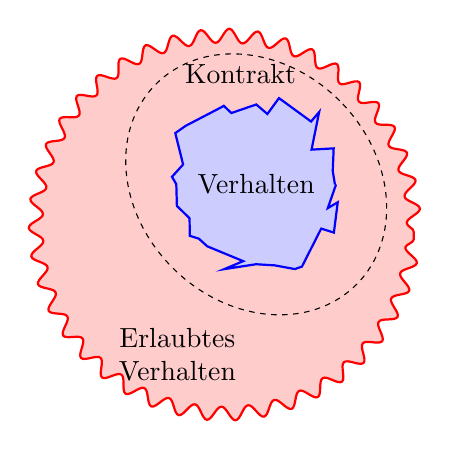
\begin{tikzpicture}
    \fill[fill=red!20,draw=red,thick] decorate[decoration={snake}] { (-0.4,-0.6) circle (2.4) };
    \fill[fill=blue!20,draw=blue,thick] decorate[decoration={random steps,segment length=2mm,amplitude=2mm}] {(0,0) circle (1)};
    \draw[dash pattern=on 2pt off 2pt,rotate=45] (0,0) ellipse (1.5 and 1.8);
    \node at (0,0) {Verhalten};
    \node at (-1,-2.2) {\begin{tabular}{c}Erlaubtes\\Verhalten\end{tabular}};
    \node at (-0.2,1.4) {Kontrakt};
  \end{tikzpicture}
  \caption{Verhalten und Kontrakte}
  \label{fig:contracts}
\end{figure}

Ist ein vereinfachender Kontrakt-Automat gefunden, so muss die formelle Verifikation zunächst beweisen, dass der Kontrakt von der ursprünglichen Komponente eingehalten wird.
Dies kann beispielsweise festgestellt werden, indem der Kontrakt in den Formalismus der Komponente übersetzt wird und dort verifiziert wird.
Ist gesichert, dass alle Kontrakte von den Komponenten erfüllt werden, so werden die Kontrakte verwendet, um das Gesamtsystem zu verifizieren.
Sind die Kontrakte allerdings zu locker formuliert, spezifizieren also mehr Verhalten als die zu verifizierende Formel erlaubt, so werden bei der Verifikation Fehler gefunden, die bei einer normalen Verifikation ohne Kontrakte nicht auftreten würden.
Eine Lösung für dieses Problem wird in Abschnitt \ref{sec:error-refinement} vorgestellt.

Die Formulierung von Kontrakten stellt einen Balance-Akt dar:
Formuliert man die Kontrakte zu scharf, so hat der resultierende Automat ähnlich viele Zustände wie die ursprüngliche Komponente und es gibt keinen Gewinn durch die Verwendung von Kontrakten.
Wird der Kontrakt jedoch zu lose formuliert so bekommt der Kontrakt-Automat viele Transitionen und zeigt Verhalten, dass die Verifikation der Systemeigenschaft unmöglich machen.

Um gute Kontrakte zu formulieren, muss der Anwender zwischen relevanten und irrelevanten Verhaltensweisen unterscheiden.
Ist beispielsweise für die zu verifizierende Eigenschaft unerheblich, welchen konkreten Wert eine Variable aufweist, sondern nur wichtig, dass der Wert eine bestimmte Eigenschaft erfüllt, so lässt sich häufig ein Kontrakt finden, der den Wert der Variable nicht-deterministisch auf einen Wert setzt.